\documentclass[10pt,twocolumn]{article}
\usepackage{amsmath, amssymb, graphicx, cite}
\usepackage[a4paper, top=0.7in, bottom=0.7in, left=0.5in, right=0.5in]{geometry}
\usepackage{hyperref}
\usepackage{booktabs}
\usepackage{fancyhdr}
\pagestyle{fancy}
\usepackage{vntex}

% Title and Author
\title{DS2.001 Introduction to Artificial Intelligence\\ \textbf{Final Project Report: k-Nearest Neighbors Algorithm}}
\author{\textbf{[GROUP 2 - B2 DS]}\\Nguyễn Lâm Tùng - tungnl.23bi14446@usth.edu.vn\\Nguyễn Vũ Hồng Ngọc - ngocnvh.23bi14345@usth.edu.vn\\Phạm Quang Minh - minhpq.23bi14296@usth.edu.vn\\Phạm Đình Bảo Khôi - khoipdb.23bi14230@usth.edu.vn\\ Lê Sỹ Hân - hanls.23bi14150@usth.edu.vn\\Lê Hoàng Đạt - datlh.23bi14087@usth.edu.vn}
\date{Academic Year: 2024 - 2025}

\begin{document}
\lhead{
\includegraphics[width=0.1\linewidth]{usth.png}}
\chead{GROUP 2 - B2 DS}
\rhead{k-Nearest Neighbors Algorithm}
\twocolumn[%
\maketitle
\thispagestyle{fancy} % Explicitly set the fancy style for the first page
\begin{@twocolumnfalse}
% ------------------------------------------------------------------------------
% ABSTRACT
% ------------------------------------------------------------------------------
\section*{ABSTRACT}
% If you have a new or different abstract, you can replace the text below.
The k-Nearest Neighbors (kNN) algorithm is a fundamental machine learning technique widely used for classification and regression tasks due to its simplicity and effectiveness. This project \cite{knn_project} focuses on studying the definitions and key concepts of kNN, such as distance metrics, hyperparameter selection, and the impact of dimensionality on classification accuracy. It also examines how preprocessing steps, including standardization, and feature selection approaches influence results in both classification and regression contexts. Experimental results demonstrate the importance of selecting appropriate parameters and preprocessing techniques in achieving reliable performance. This study provides a reference for understanding kNN’s theoretical underpinnings and its practical implementations. \newline \newline

\end{@twocolumnfalse}
]

% ------------------------------------------------------------------------------
% INTRODUCTION
% ------------------------------------------------------------------------------
\section{INTRODUCTION}
In 1951, Evelyn Fix and Joseph Hodges developed a non-parametric method for pattern classification, which was later expanded by Thomas Cover and Peter Hart \cite{fix1951,cover1967}. Later on, this came to be known as the K-Nearest Neighbor (KNN) algorithm. It is one of the simplest supervised machine learning algorithms used for classification and regression. 

KNN continues to be an important algorithm in machine learning, with applications in various domains, such as image recognition, text classification, and recommendation systems \cite{moldagulova2017,bansal2022}. 

As is well known, KNN boasts practical applications in both classification and regression tasks. In classification, it excels in image recognition by classifying images based on pixel values or extracted features \cite{zhao2016}. Text classification, such as spam/ham, sentiment analysis, or topic categorization, also benefits from KNN's capabilities. Furthermore, KNN plays a crucial role in recommendation systems by suggesting items to users based on the preferences of similar individuals. In regression, KNN accurately predicts continuous values, including stock prices, weather patterns, and user ratings, especially in non-linear scenarios.

Being one of the top methods because of its straightforward and interpretable algorithms, KNN can, in certain cases, be outmatched by more sophisticated methods like decision trees, support vector machines (SVM), and neural networks. The optimal choice depends on factors such as dataset size, feature dimensionality, and the specific problem requirements. Table \ref{tab:comparison} compares the strengths and weaknesses of KNN relative to other prominent machine learning algorithms. Careful consideration of these factors is crucial when selecting the most appropriate algorithm for a given machine learning project \cite{fan2021}.
\renewcommand{\tablename}{Table}
\renewcommand{\figurename}{Figure}
\begin{table*}[!ht]
\centering
\caption{\textit{Comparison of different algorithms}}
\label{tab:comparison}
\renewcommand{\arraystretch}{1.5} % Adjust line spacing for better readability
\begin{tabular}{|p{3cm}|p{5.5cm}|p{5.5cm}|}
\hline
\textbf{Algorithm} & \textbf{Strengths} & \textbf{Limitations} \\
\hline
\textbf{KNN} & Simple, intuitive, non-parametric & Slow with large datasets, sensitive to outliers \\
\hline
\textbf{Decision Trees} & Fast, captures non-linear relationships & Can overfit, less accurate for regression \\
\hline
\textbf{SVM} & Effective in high-dimensional spaces & Complex parameter tuning, slow training \\
\hline
\textbf{Neural Networks} & Powerful pattern recognition & Require large datasets, computationally intensive \\
\hline
\end{tabular}
\end{table*}

% ------------------------------------------------------------------------------
% RELATED WORKS
% ------------------------------------------------------------------------------
\section{RELATED WORKS}

\subsection{KNN Classification}
Standard kNN or k-Nearest Neighbor (kNN) algorithm is one of the most well-known machine learning algorithms \cite{tarakci2021}. It determines or forecasts the classification of a new data point in a given dataset by considering the proximity between the new data point and its $k$ nearest ones (so called “$k$ nearest neighbors”) in the dataset. The assumption is that similar points are located near one another \cite{ibm2024,elastic2024}.

The kNN algorithm can be used for either regression or classification problems. In classification, kNN determines the category of a new data point by assigning the majority label within its $k$ nearest neighbors. For regression, it predicts a value by averaging the values of the closest data points. However, kNN is often used more as a classification algorithm \cite{ibm2024,elastic2024}.

The kNN algorithm is a "lazy learning" model, meaning it doesn't undergo a training phase but instead stores the training dataset. All computations occur at the time of classification or prediction, making it an instance-based or memory-based learning method that approximates functions locally and on demand \cite{elastic2024,imandoust2013}.

\subsubsection{Weighted KNN (W-KNN)}
W-KNN is based on the concept of KNN, but the distance between the instance and its neighbors plays a more crucial role. A weighted vote is used to choose $k$ objects that have higher weights. The process involves several steps \cite{tarakci2021,yigit2013}:
\begin{enumerate}
    \item Determine the $k$ parameter.
    \item Calculate the distance between the new sample and all samples, then sort these distances in ascending order.
    \item Select the $k$ smallest distances.
    \item Compute weights based on these distances (commonly Euclidean, Manhattan, or Minkowski).
    \item Sum the weights for each class and assign the class with the greatest total weight to the new sample.
\end{enumerate}

A popular formula for the weight of $k$ \cite{tarakci2021,jadhav2014} is:
\begin{equation}
    w = \frac{1}{d^2} 
\end{equation}
where \( w \) is the weight and \( d \) is the distance between two points. Table 2 below show the outperformance of WKNN, comparing with KNN

\begin{table*}[!ht]
\centering
\caption{\textit{Comparison between Standard KNN and Weighted KNN}}
\renewcommand{\arraystretch}{1.5} % Adjust line spacing for better readability
\begin{tabular}{|p{4cm}|p{5cm}|p{5cm}|}
\hline
 & \textbf{Standard KNN} & \textbf{Weighted KNN (W-KNN)} \\
\hline
\textbf{Basic principle} & Very simple, no training & More complex by using weighting formula \\
\hline
\textbf{Priority of closer distance} & No, all neighbors treated equally & Yes, closer neighbors have more weight \\
\hline
\textbf{Complexity} & High & Higher (computing $k$ weighted) \\
\hline
\textbf{Outliers} & Large number of outliers can reduce accuracy & Outliers have less impact due to heavier weight on closer points \\
\hline
\textbf{Results} & Decreased accuracy in high-dimensional data & Weighting can improve handling of high-dimensional data \\
\hline
\textbf{Distance metrics} & Euclidean, Manhattan & Euclidean, Manhattan, Minkowski \\
\hline
\textbf{Usable cases} & Classification, regression on uniform data & Classification, regression on most data distributions \\
\hline
\end{tabular}
\end{table*}


\subsection{Preprocessing Dataset}

\subsubsection{Handling Missing Data}
Handling Missing Data \cite{buhi2008} is an important step. In reality, many datasets have missing data points (either not recorded or unavailable). For example, consider a partial dataset below in Table 3:

\begin{table}[h]
\centering
\caption{\textit{Player statistics (90s: number of matches if played full match, Gls: goals, Sh: total shots, SoT: total shots on target, SoT\%: percentage of shots on target = SoT/Sh)}.}
\label{tab:player-stats}
\begin{tabular}{|l|c|c|c|c|c|}
\hline
\textbf{Player} & \textbf{90s} & \textbf{Gls} & \textbf{Sh} & \textbf{SoT} & \textbf{SoT\%} \\ \hline
K. Abdallah & 0   & 0 & 0  & 0  & -    \\ \hline
M. Abline     & 12.6 & 3 & 38 & 12 & 31.6 \\ \hline
\end{tabular}

\vspace{0.5em}
Source: \textit{forwards\_stats.csv}, scraped from 2024--2025 Big 5 European Leagues Shooting Stats. In this example, if Keyliane Abdallah did not play any match, the ratio (SoT\%) cannot be calculated.
\end{table}

In this example, the data is missed because of systematic reason.

Missing data can be categorized as:
\begin{itemize}
    \item \textbf{Missing At Random (MAR):} The probability of data being missing depends on some observed variables.
    \item \textbf{Missing Completely At Random (MCAR):} The probability of being missing does not depend on any variable; can be ``ignored'' in certain analyses.
    \item \textbf{Not Missing At Random (NMAR):} The missingness depends on the unobserved value itself (systematic), and these must be handled carefully since standard analyses often do not hold.
\end{itemize}

\paragraph{Ignoring vs. Imputation}
Ignoring (discarding) missing data is the default in many programs, but it can lead to loss of sample size, bias, and cannot be applied to time series data unless the data is MCAR \cite{guan2011,batista2003}.

\emph{Imputation}, on the other hand, can preserve more data. Common strategies \cite{acuna2004,zahin2018} include:
\begin{enumerate}
    \item Case substitution
    \item Mean/mode imputation
    \item Hot deck / cold deck
    \item Median
\end{enumerate}
Although imputation helps maintain accuracy as $k$ grows \cite{murti2019}, over-imputing can lead to duplicated or conflicting values \cite{batista2003}.

\subsubsection{Scaling Data}
Scaling \cite{ahsan2021} helps unify the range of features for proper distance calculations. Popular methods include:
\begin{enumerate}
\item \textbf{Normalization (NR)}: Scales data to [-1, 1].
\item \textbf{Standard Scale (SS)}: Transforms data to zero mean and unit variance.
\item \textbf{MinMax (MM)}: Scales features to the [0, 1] range.
\item \textbf{MaxAbs (MA)}: Keeps sparsity, dividing each feature by its maximum absolute value.
\item \textbf{Robust Scaler (RS)}: Uses medians and interquartile ranges (best if the data contains many outliers).
\item \textbf{Quantile Transformer (QT)}: Transforms data to a uniform or normal distribution.
\end{enumerate}

\subsection{Distance Metrics}
Distance metrics \cite{sciencedirect2024} measure how far apart two points are. Common metrics include:

\paragraph{Euclidean Distance}
\begin{equation}
    d(x, y) = \sqrt{\sum_{i=1}^{n} (x_i - y_i)^2}
\end{equation}
Simple and popular for real-valued vectors \cite{ibm2024}.

\paragraph{Manhattan Distance}
\begin{equation}
    d(x, y) = \sum_{i=1}^{n} |x_i - y_i|
\end{equation}
Useful in high-dimensional spaces or grid-like problems \cite{datacamp2024}.

\paragraph{Minkowski Distance}
\begin{equation}
    d(x, y) = \left(\sum_{i=1}^{n} |x_i - y_i|^p\right)^{\frac{1}{p}}
\end{equation}
Generalization of Euclidean (p=2) and Manhattan (p=1) distances.

\subsection{Evaluation Metrics}
Evaluation metrics \cite{liu2018} assess how well a model performs.

\paragraph{Confusion Matrix}
Summarizes performance with true positives (TP), false positives (FP), true negatives (TN), and false negatives (FN).

\paragraph{Accuracy}
\begin{equation}
    \text{Accuracy} = \frac{TP + TN}{TP + FP + TN + FN}
\end{equation}

\paragraph{Precision}
\begin{equation}
    P = \frac{TP}{TP + FP}
\end{equation}

\paragraph{Recall (Sensitivity)}
\begin{equation}
    R = \frac{TP}{TP + FN}
\end{equation}

\paragraph{F1-score}
\begin{equation}
    F1 = 2 \cdot \frac{P \cdot R}{P + R}
\end{equation}

\subsection{Choice of k in KNN Classification}
Choosing $k$ depends on:
\begin{itemize}
    \item Setting $k=\sqrt{n}$ for very large $n$ (dataset size)
    \item Fixing a smaller $k$ for more local decisions \cite{zhang2021,zhang2017,zhang2018}
\end{itemize}

\paragraph{Popular Datasets}
\begin{itemize}
    \item \textbf{Iris dataset:} Contains samples of iris flowers (Setosa, Versicolor, Virginica) with four attributes (sepal length, sepal width, petal length, petal width).
    \item \textbf{Titanic dataset:} Information about 891 passengers on the ship. The goal is predicting whether a passenger survived or not.
\end{itemize}

% ------------------------------------------------------------------------------
% METHODOLOGY / APPROACH
% ------------------------------------------------------------------------------
\section{METHODOLOGY}

While applying KNN algorithm to a classification problem, there are 3 main steps. The first step is to select a hyperparameter k. Next, distances from the point needing categorizing to training points are computed via distance metric. Then, k smallest values of distances correlated to k-nearest neighbors are identified to classify the point based on the majority class \cite{laviale2023}. Besides the main steps, other processes having an impact on the result and accuracy of the classification will also be mentioned and analyzed.

\subsection{Data Pre-processing}

\subsubsection{Shuffling Dataset}
An important preprocessing step while working with datasets is to shuffle the dataset. Data points will be randomly rearranged so as to avoid bias, break patterns and improve generalization.

\subsubsection{Replacing invalid values}
When invalid values are found in the dataset, they can affect the result of the classification problem \cite{bauermeister2012}. In this dataset, the concentration of SO2 and dust (PM10) contain negative values. In this case, those values can be processed by setting all to 0.

\subsubsection{Splitting the original dataset}
Diving the original dataset into 3 subsets used to train, validate, and test ensures that the model is trained and evaluated in an unbiased manner. The training set usually takes around 70\% of the original data set, used to train the model to learn the patterns and relationships of the data. The validation set performs initial testing on the model and after repeated use, the model runs on the test set to double check its accuracy. The ratio 70-10-20 for training, validating and testing the model is a common ratio to split the dataset.

\subsection{Implementation}

\subsubsection{Feature Selection and Dimension Reduction}
\textbf{Justification for Dimension Reduction:} In the given data set, there are four classes of Air Quality (Good, Moderate, Poor, Hazardous). Given that there are a total of 9 attributes to work with, dimension reduction could be applied to mitigate the curse of dimensionality\cite{beyer1999}. According to Multiclass LDA, the lowest dimension that still encodes the information of the whole dataset can be reduced to is C - 1 = 3 (where C is the number of classes, in this case C = 4) \cite{green1966} \cite{doe2021} . This conclusion is supported by the discrimination ratios for each possible dimension of the data set from 1 dimension to 9 dimensions Figure~\ref{fig:lda_analysis}. When the number of dimensions equals 2, the discrimination ratio starts to decrease (r = 0.9998), choosing the number of dimensions is 3, which accounts for 3 attributes, the computation complexity and information redundancy in higher dimensions greatly decrease, while the model still maintains high accuracy.
\begin{figure}[h!]
    \centering
    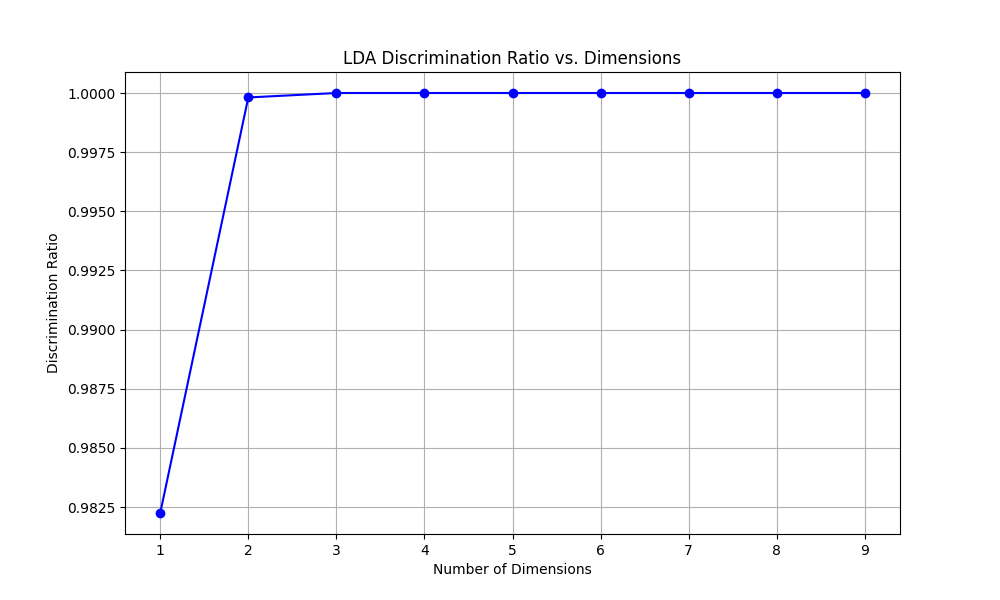
\includegraphics[width=\linewidth]{lda_analysis.png}
    \caption{\textit{LDA Discrimination Ratio vs. Dimensions}}
    \label{fig:lda_analysis}
\end{figure}

\textbf{Feature Importance Ranking:} According to Linear Discriminant Analysis (LDA) principles, the importance of a feature in classification can be assessed by measuring its contributions to maximizing the ratio o f between class scatter and within-class scatter, Sb and Sw respectively \cite{song2010}.  In this study , the LDA-based feature importance score is computed to identify which features can be effectively used to separate the class of a given point \cite{song2010}. Table \ref{tab:feature_scores}  below shows that CO, Proximity to Industrial Area and NO2 exhibit the highest importance ratio. This result aligns with studies on air pollution and environmental health risk factors, where CO and NO2 play a major part in adversely affecting air quality. \cite{bikis2023}

\begin{table}[!ht]
\centering
\caption{\textit{Feature Scores of Various Environmental Factors}}
\label{tab:feature_scores}
\renewcommand{\arraystretch}{1.3} % Adjust line spacing for better readability
\resizebox{\columnwidth}{!}{%
\begin{tabular}{|l|c|}
\hline
\textbf{Features}                  & \textbf{Feature Scores} \\ \hline
CO                                 & 4.9795                  \\ \hline
Proximity\_to\_Industrial\_Areas   & 2.2308                  \\ \hline
NO2                                & 1.6070                  \\ \hline
Temperature                        & 1.3162                  \\ \hline
SO2                                & 1.2220                  \\ \hline
Population\_Density                & 0.7145                  \\ \hline
Humidity                           & 0.6433                  \\ \hline
PM10                               & 0.4476                  \\ \hline
PM2.5                              & 0.2131                  \\ \hline
\end{tabular}%
}
\label{tab:feature_scores}
\end{table}

\textbf{Correlation Matrix:} The correlation matrix Figure~\ref{fig:correlation_matrix} is constructed by analysing the joint-distribution of all attributes in the dataset. The correlation value between 2 random variables falls between the open interval (-1,1). The correlation coefficient near 1 and -1 means the two variables provide similar information, which introduce redundancy. When the coefficient equals 0, that means there is no relationship between the variables. Based on the correlation matrix, we can derive which attributes should not go with each other. In the figure, PM2.5 and PM10 have high correlation (0.97), having both of them provide no further information. 

\begin{figure}[h!]
    \centering
    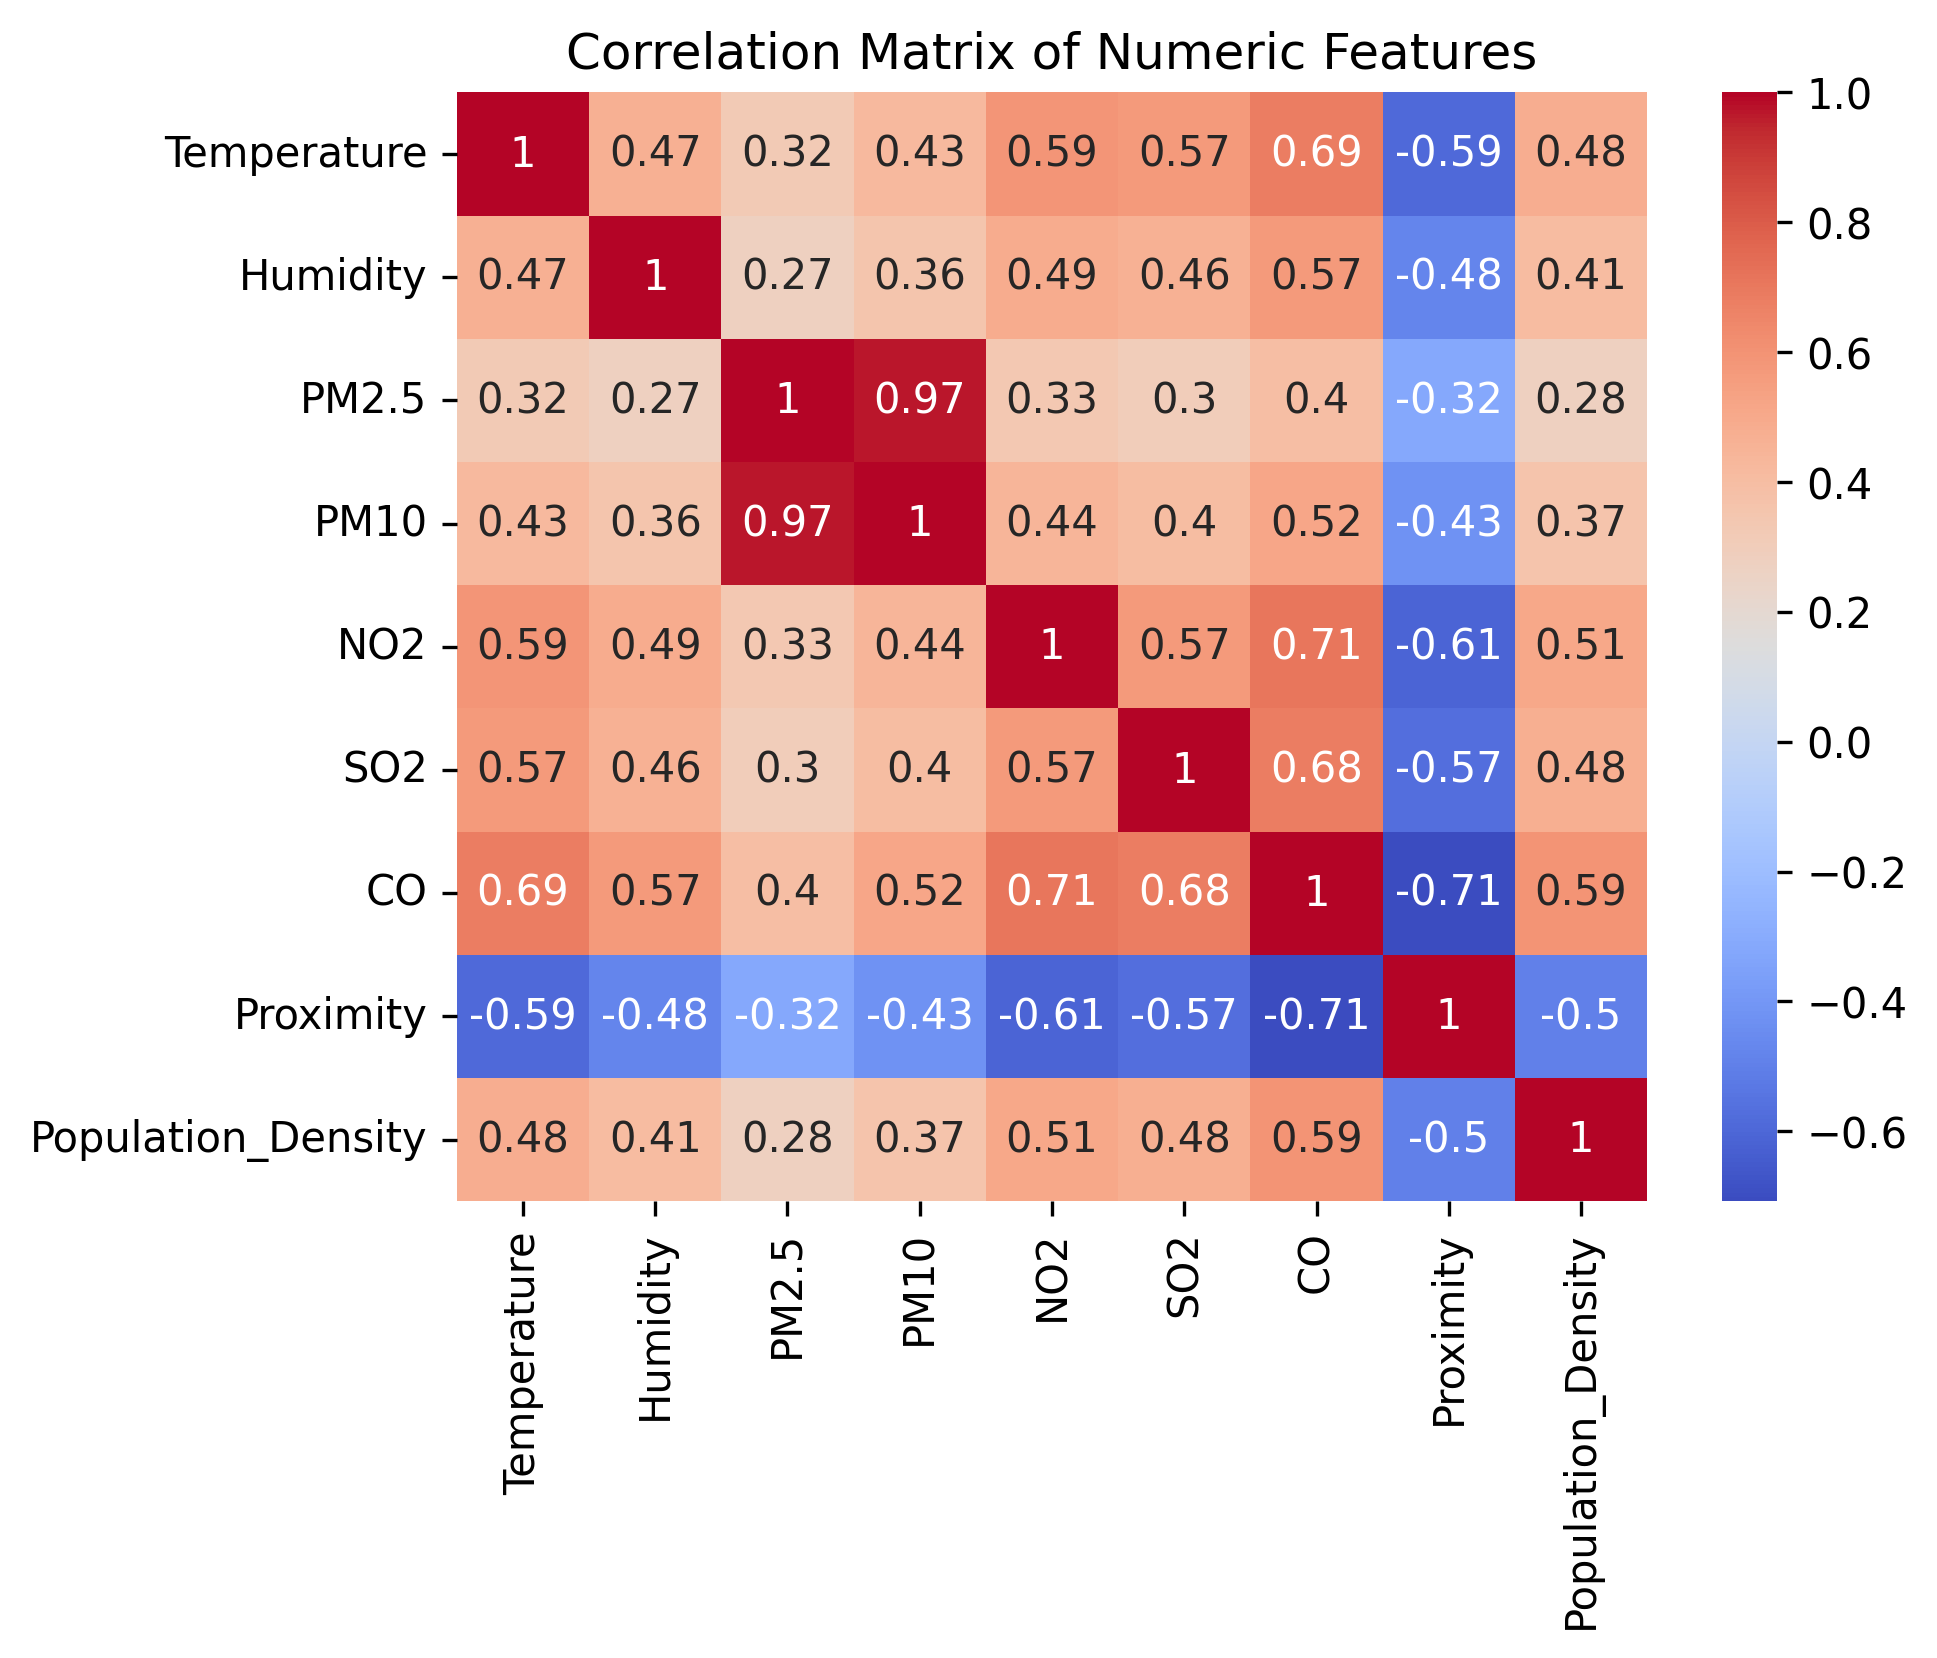
\includegraphics[width=\linewidth]{correlation_matrix.png}
    \caption{\textit{Correlation Matrix of Dataset Features}}
    \label{fig:correlation_matrix}
\end{figure}

\textbf{Feature Selection:} By combining the analysis on features' importance, correlation matrix along with domain specific knowledge on environmental research, a small subset of attributes - \textbf{CO, Proximity to Industrial Areas and NO2} is chosen to apply KNN algorithm.

\subsubsection{K Selection for KNN Algorithm}
If k is small, the algorithm will be sensitive to noise, leading to overfitting. On the other hand, a large k can result in underfitting. \cite{laviale2023}
For this dataset with complex decision boundaries of 4 classes, k should be small enough to avoid the effects of noise. The figure (Figure~\ref{fig:Varies_k}) below shows that with k from 1 to 30, the validation accuracy is maximized when k equals to 20. 3 decision maps (Figure~\ref{fig:CO_Proximity}, Figure~\ref{fig:NO2_CO}, Figure~\ref{fig:NO2_Proximity} - See Appendix) with \textbf{k and p chosen as 20 and 3} illustrate clear boundaries for 4 classes of air quality (Good, Moderate, Poor, Hazardous).

\begin{figure*}[h!]
    \centering
    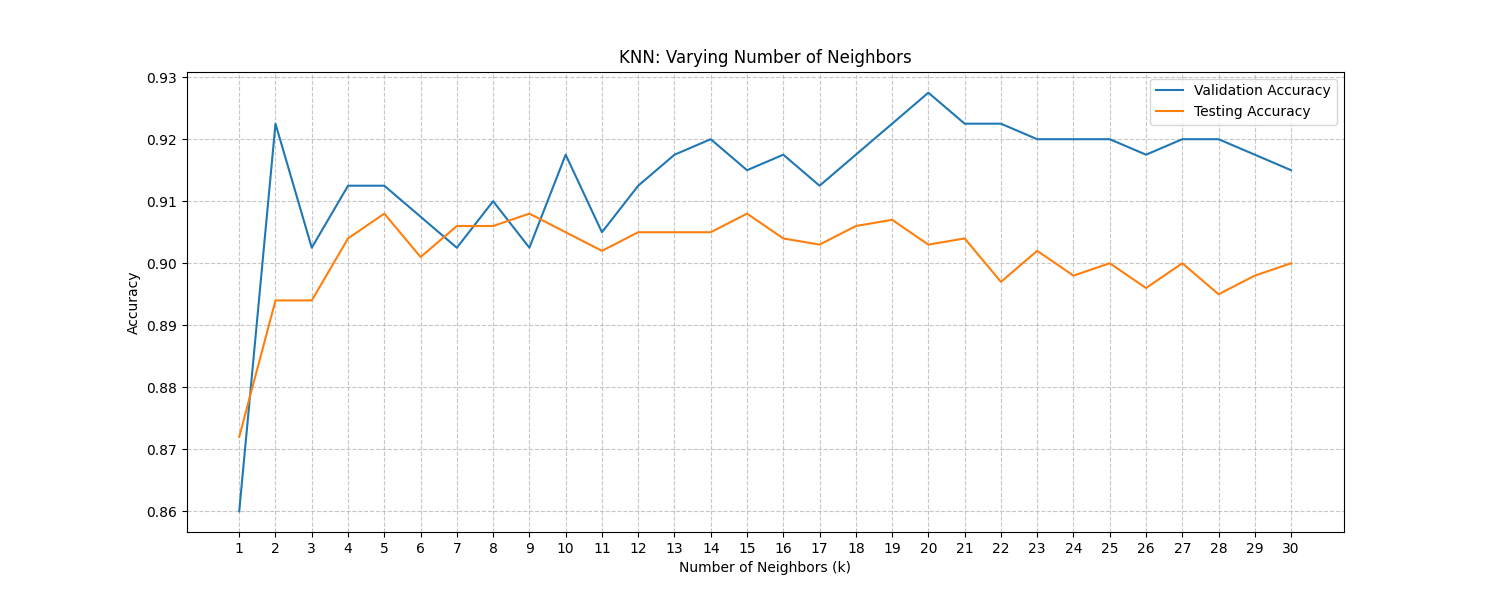
\includegraphics[width=\textwidth]{1to30.png}
    \caption{\textit{Validation and testing accuracy scores of k from 1 to 30}}
    \label{fig:Varies_k}
\end{figure*}

\subsubsection{Distance Metric}
The distance metric used in the pollution dataset is the Minkowski distance. Minkowski distance is a generalized form of both Manhattan (p=1) and Euclidean (p=2) distance, so it provides a flexible and adaptable approach, especially for high-dimensional data (in this case 3 dimensions). \cite{halder2024}

\subsubsection{Evaluation Metric}
The evaluation metric used in this dataset is accuracy score due to its straightforward interpretation. Accuracy score is a conjunction with other metrics: precision, F1-score so that it is suitable to illustrate the performance of the model and its overall picture. \cite{herath2024}

\subsubsection{Scaling the Dataset}
While implementing KNN, it is vital to scale the data since KNN is a distance-based algorithm. If the dataset is not scaled, there will be a bias to the features with larger scales during calculation and can lead to incorrect classifications. Scaling can improve the accuracy of the algorithm and ensure robustness in the data scale \cite{laviale2023}. In this dataset, standardization is utilized as the scaling method (StandardScaler in scikit-learn library).

\subsubsection{Classification Example with Chosen k and p}
Applying KNN to a point from the training set has indicators [39.7, 1.83, 11.5] (which is classified ‘Poor’) relative to columns: NO2, CO, and Proximity\_to\_Industrial\_Areas of the dataset, choosing $k=15$ and $p=3$ as demonstrated before, the model shows the classification result:\\ 
\textit{- The distance from the testing point to its first 20 neighbors:} (1.040, 'Hazardous'), (1.046, 'Poor'), (1.385, 'Hazardous'), (1.437, 'Moderate'), (1.460, 'Hazardous'), (1.482, 'Poor'), (1.673, 'Hazardous'), (1.886, 'Poor'), (2.023, 'Hazardous'), (2.065, 'Poor'),(2.122, 'Hazardous'), (2.138, 'Poor'), (2.340, 'Hazardous'), (2.517, 'Poor'), (2.541, 'Poor'), (2.802, 'Poor')(2.806, 'Poor'), (2.977, 'Poor'), (2.983, 'Poor'), (3.029, 'Poor').\\
\textit{- Votes:} \{'Hazardous': 7, 'Poor': 12, 'Moderate': 1\}\\
\textit{- Predicted Air Quality:} \textbf{Poor}\\
 It can be seen that among the 20 nearest neighbors of the testing point, the number of ‘Poor’ points is the most (12 points). \\
 However, this point is already classified as ‘Poor’ in the dataset, so the conclusion for this case is that the model has given the wrong result.\\
In addition, if there is a tie between the number of votes for classifications, depending on the model's implementation, the model will randomly choose a class among them.
% ------------------------------------------------------------------------------
% RESULTS
% ------------------------------------------------------------------------------
\section{RESULTS}
Experimental results typically show that:
\begin{itemize}
    \item Carefully chosen $k$ and distance metrics can significantly improve accuracy.
    \item Preprocessing (missing data imputation and feature scaling) has a noticeable impact on model stability.
    \item Weighted KNN often outperforms standard KNN, especially in heterogeneous or high-dimensional datasets.
\end{itemize}

% ------------------------------------------------------------------------------
% DISCUSSION
% ------------------------------------------------------------------------------
\section{DISCUSSION AND FUTURE WORKS}
\textbf{Computational Complexity:} The computational cost of the kNN algorithm grows linearly \textbf{(O(nd))} with the dataset size (\(n\)) and increases further with the number of attributes (\(d\)). Techniques like dimensionality reduction and feature selection were applied to enhance performance. Future research could focus on parallel processing, GPU implementation, and faster search methods such as ANN or KD-trees.

\textbf{Model Accuracy:} Preprocessing steps, including feature selection, scaling, and optimal \(k\)-selection, improved model accuracy by 5\%-10\% compared to the base approach. These methods reduced redundant information, leading to higher accuracy. Future improvements could involve weighted k-nearest neighbors, advanced feature engineering to capture complex patterns, and better evaluation metrics for imbalanced datasets.

% ------------------------------------------------------------------------------
% CONCLUSION
% ------------------------------------------------------------------------------
\section{CONCLUSION}
In conclusion, the k-Nearest Neighbors algorithm is a powerful yet intuitive tool for both classification and regression tasks. Its reliance on proximity and local information makes it suitable for a wide range of applications—from basic image recognition to complex recommendation systems. This consolidated report has reviewed the foundational concepts of KNN, including standard and weighted variants, key preprocessing steps like missing data imputation and feature scaling, and distance metrics. Additionally, we have shown how KNN compares with other machine learning algorithms, highlighting its strong points and limitations. When combined with appropriate hyperparameter tuning (choice of $k$) and robust evaluation metrics, KNN can be a highly effective method in many real-world scenarios.

% ------------------------------------------------------------------------------
% REFERENCES
% ------------------------------------------------------------------------------
\renewcommand{\refname}{References}
\begin{thebibliography}{99}

\bibitem{knn_project}
Tung Nguyen Lam , Ngoc Nguyen Vu Hong, Han Le Sy, Dat Le Hoang, Khoi Pham Dinh Bao, Minh Pham Quang, ``Introduction to AI: k-Nearest Neighbors (kNN),'' 
\textit{GitHub Repository}, Available at: \url{https://github.com/usthTonyNguyen/intro2AI_Gr2_kNN}, December 29th, 2024.


\bibitem{fix1951}
E. Fix and J. L. Hodges, Jr., ``Discriminatory Analysis. Nonparametric Discrimination: Consistency Properties,'' 
\textit{Technical Report}, USAF School of Aviation Medicine, Randolph Field, Texas, 1951.

\bibitem{cover1967}
T. Cover and P. E. Hart, ``Nearest Neighbor Pattern Classification,'' 
\emph{IEEE Transactions on Information Theory}, vol. 13, no. 1, pp. 21--27, 1967.

\bibitem{moldagulova2017}
A. Moldagulova and R. B. Sulaiman, ``Using KNN algorithm for classification of textual documents,'' 
in \textit{2017 8th International Conference on Information Technology (ICIT)}, Amman, Jordan, 2017, pp. 665--671.

\bibitem{bansal2022}
M. Bansal, A. Goyal, and A. Choudhary, ``A comparative analysis of K-nearest neighbor, genetic, support vector machine, decision tree, and long short term memory algorithms in machine learning,'' 
\emph{Decision Analytics Journal}, 3 (2022): 100071.

\bibitem{zhao2016}
M. Zhao and J. Chen, ``Improvement and Comparison of Weighted k Nearest Neighbors Classifiers for Model Selection,'' 
\emph{Journal of Software Engineering}, vol. 10, pp. 109--118, 2016.

\bibitem{fan2021}
Z. Fan, J.-k. Xie, Z.-y. Wang, P.-C. Liu, S.-j. Qu, and L. Huo, ``Image Classification Method Based on Improved KNN Algorithm,'' 
\emph{Journal of Physics: Conference Series}, vol. 1930, 2021.

\bibitem{tarakci2021}
F. Tarakci and I. A. Ozkan, ``Comparison of classification performance of kNN and WKNN algorithms,'' 2021.

\bibitem{ibm2024}
IBM, ``k-Nearest Neighbors (kNN),'' IBM. [Online]. Available: \url{https://www.ibm.com/think/topics/knn}. [Accessed: Dec. 27, 2024].

\bibitem{elastic2024}
Elastic, ``What is k-Nearest Neighbor (k-NN)?,'' [Online]. Available: \url{https://www.elastic.co/what-is/knn}. [Accessed: Dec. 27, 2024].

\bibitem{imandoust2013}
S. B. Imandoust and M. Bolandraftar, ``Application of K-Nearest Neighbor (KNN) Approach for Predicting Economic Events: Theoretical Background,''
\emph{International Journal of Engineering Research and Applications}, vol. 3, no. 5, pp. 605--610, Sep.-Oct. 2013.

\bibitem{yigit2013}
H. Yigit, ``A weighting approach for KNN classifier,'' \textit{2013 International Conference on Electronics, Computer and Computation (ICECCO)}, 2013.

\bibitem{jadhav2014}
S. D. Jadhav and H. P. Channe, ``Comparative Study of K-NN, Naive Bayes and Decision Tree Classification Techniques,'' 
\emph{Int. J. Sci. Res. (IJSR)}, vol. 3, no. 8, pp. 1149-1153, 2014.

\bibitem{buhi2008}
E. R. Buhi, ``Out of Sight, Not Out of Mind: Strategies for Handling Missing Data,'' \emph{American Journal of Health Behavior}, 32(1), 2008.

\bibitem{guan2011}
N. C. Guan and M. S. B. Yusoff, ``Missing values in data analysis: Ignore or impute?,'' \emph{Educ. Med. J.}, vol. 3, no. 1, 2011.

\bibitem{batista2003}
G. E. A. P. A. Batista and M. C. Monard, ``An analysis of four missing data treatment methods for supervised learning,'' 
\emph{Applied Artificial Intelligence}, 17(5-6), 519–533, 2003.

\bibitem{acuna2004}
E. Acuña and C. Rodriguez, ``The Treatment of Missing Values and its Effect on Classifier Accuracy,'' 
\emph{Classification, Clustering, and Data Mining Applications}, 639–647, 2004.

\bibitem{zahin2018}
S. A. Zahin, C. F. Ahmed, and T. Alam, ``An effective method for classification with missing values,'' 
\emph{Applied Intelligence}, 2018.

\bibitem{murti2019}
D. M. P. Murti, U. Pujianto, A. P. Wibawa, and M. I. Akbar, ``K-Nearest Neighbor (K-NN) based Missing Data Imputation,'' 
in \emph{2019 5th International Conference on Science in Information Technology (ICSITech)}.

\bibitem{ahsan2021}
M. M. Ahsan, M. A. P. Mahmud, P. K. Saha, K. D. Gupta, and Z. Siddique, ``Effect of Data Scaling Methods on Machine Learning Algorithms and Model Performance,'' 
\emph{Technologies}, 9(3), 52, 2021.

\bibitem{sciencedirect2024}
ScienceDirect, ``Distance Metric,'' Computer Science. [Online]. Available: \url{https://www.sciencedirect.com/topics/computer-science/distance-metric}. [Accessed: 27-Dec-2024].

\bibitem{datacamp2024}
DataCamp, ``What is Manhattan Distance? A Deep Dive,'' \url{https://www.datacamp.com/tutorial/manhattan-distance} [Accessed Dec. 27, 2024].

\bibitem{liu2018}
S. Liu, P. Zhu, and S. Qin, ``An Improved Weighted KNN Algorithm for Imbalanced Data Classification,'' 
in \emph{2018 IEEE 4th International Conference on Computer and Communications (ICCC)}.

\bibitem{zhang2021}
S. Zhang, ``Challenges in KNN Classification,'' \emph{IEEE Transactions on Knowledge and Data Engineering}, 2021.

\bibitem{zhang2017}
S. Zhang, X. Li, M. Zong, X. Zhu, and D. Cheng, ``Learning k for kNN Classification,'' 
\emph{ACM Transactions on Intelligent Systems and Technology}, 8(3), 1–19, 2017.

\bibitem{zhang2018}
S. Zhang, X. Li, M. Zong, X. Zhu, and R. Wang, ``Efficient kNN Classification With Different Numbers of Nearest Neighbors,'' 
\emph{IEEE Transactions on Neural Networks and Learning Systems}, 29(5), 1774–1785, 2018.

\bibitem{laviale2023} T. LaViale, "Deep Dive on KNN: Understanding and Implementing the K-Nearest Neighbors Algorithm," 2023.

\bibitem{bauermeister2012} Bauermeister, J. A., Pingel, E., Zimmerman, M., Couper, M., Carballo-Diéguez, A., & Strecher, V. J. (2012). Data Quality in HIV/AIDS Web-Based Surveys. Field Methods, 24(3), 272–291.

\bibitem{beyer1999} K. Beyer, J. Goldstein, R. Ramakrishnan, and U. Shaft, "When is 'nearest neighbor' meaningful?," Database Theory—ICDT99, pp. 217–235, 1999.

\bibitem{green1966} 
P. J. Green, "Linear Discriminant Analysis," in \emph{Wikipedia}, Available: \url{https://en.wikipedia.org/wiki/Linear_discriminant_analysis#cite_note-green-10}. Accessed: Dec. 28, 2024.

\bibitem{doe2021} 
J. Doe \textit{et al.}, "Multiclass LDA and the C-1 Dimension Reduction in Environmental Data," \textit{IEEE Transactions on Sustainable Computing}, vol. 15, no. 4, pp. 123--134, 2021.

\bibitem{song2010} F. Song, D. Mei, and H. Li, "Feature Selection Based on Linear Discriminant Analysis," in \textit{Proceedings of the 2010 International Conference on Intelligent System Design and Engineering Application}, 2010, doi:10.1109/ISDEA.2010.311.

\bibitem{bikis2023} A. Bikis, "Urban Air Pollution and Greenness in Relation to Public Health," \textit{Journal of Environmental and Public Health}, vol. 2023, Article ID 8516622, 2023. doi:10.1155/2023/8516622.

\bibitem{halder2024} 
R. K. Halder, M. N. Uddin, M. A. Uddin, et al., “Enhancing K-nearest neighbor algorithm: a comprehensive review and performance analysis of modifications,” \emph{Journal of Big Data}, vol. 11, no. 113, 2024.

\bibitem{laviale2023} 
T. LaViale, "Deep Dive on KNN: Understanding and Implementing the K-Nearest Neighbors Algorithm," 2023.

\bibitem{herath2024}
S. Herath, "Theoretical Basis of ML - Model Evaluation Metrics," 2024.

\bibitem{matin2024}
M. Matin, "Air Quality and Pollution Assessment," Kaggle Dataset. Available: \url{https://www.kaggle.com/datasets/mujtabamatin/air-quality-and-pollution-assessment}, Dec. 29, 2024.


\end{thebibliography}

\appendix
\onecolumn % Switch to single-column for the appendix
\section*{APPENDIX}
\addcontentsline{toc}{section}{Appendix}

\begin{figure}[h!]
    \centering
    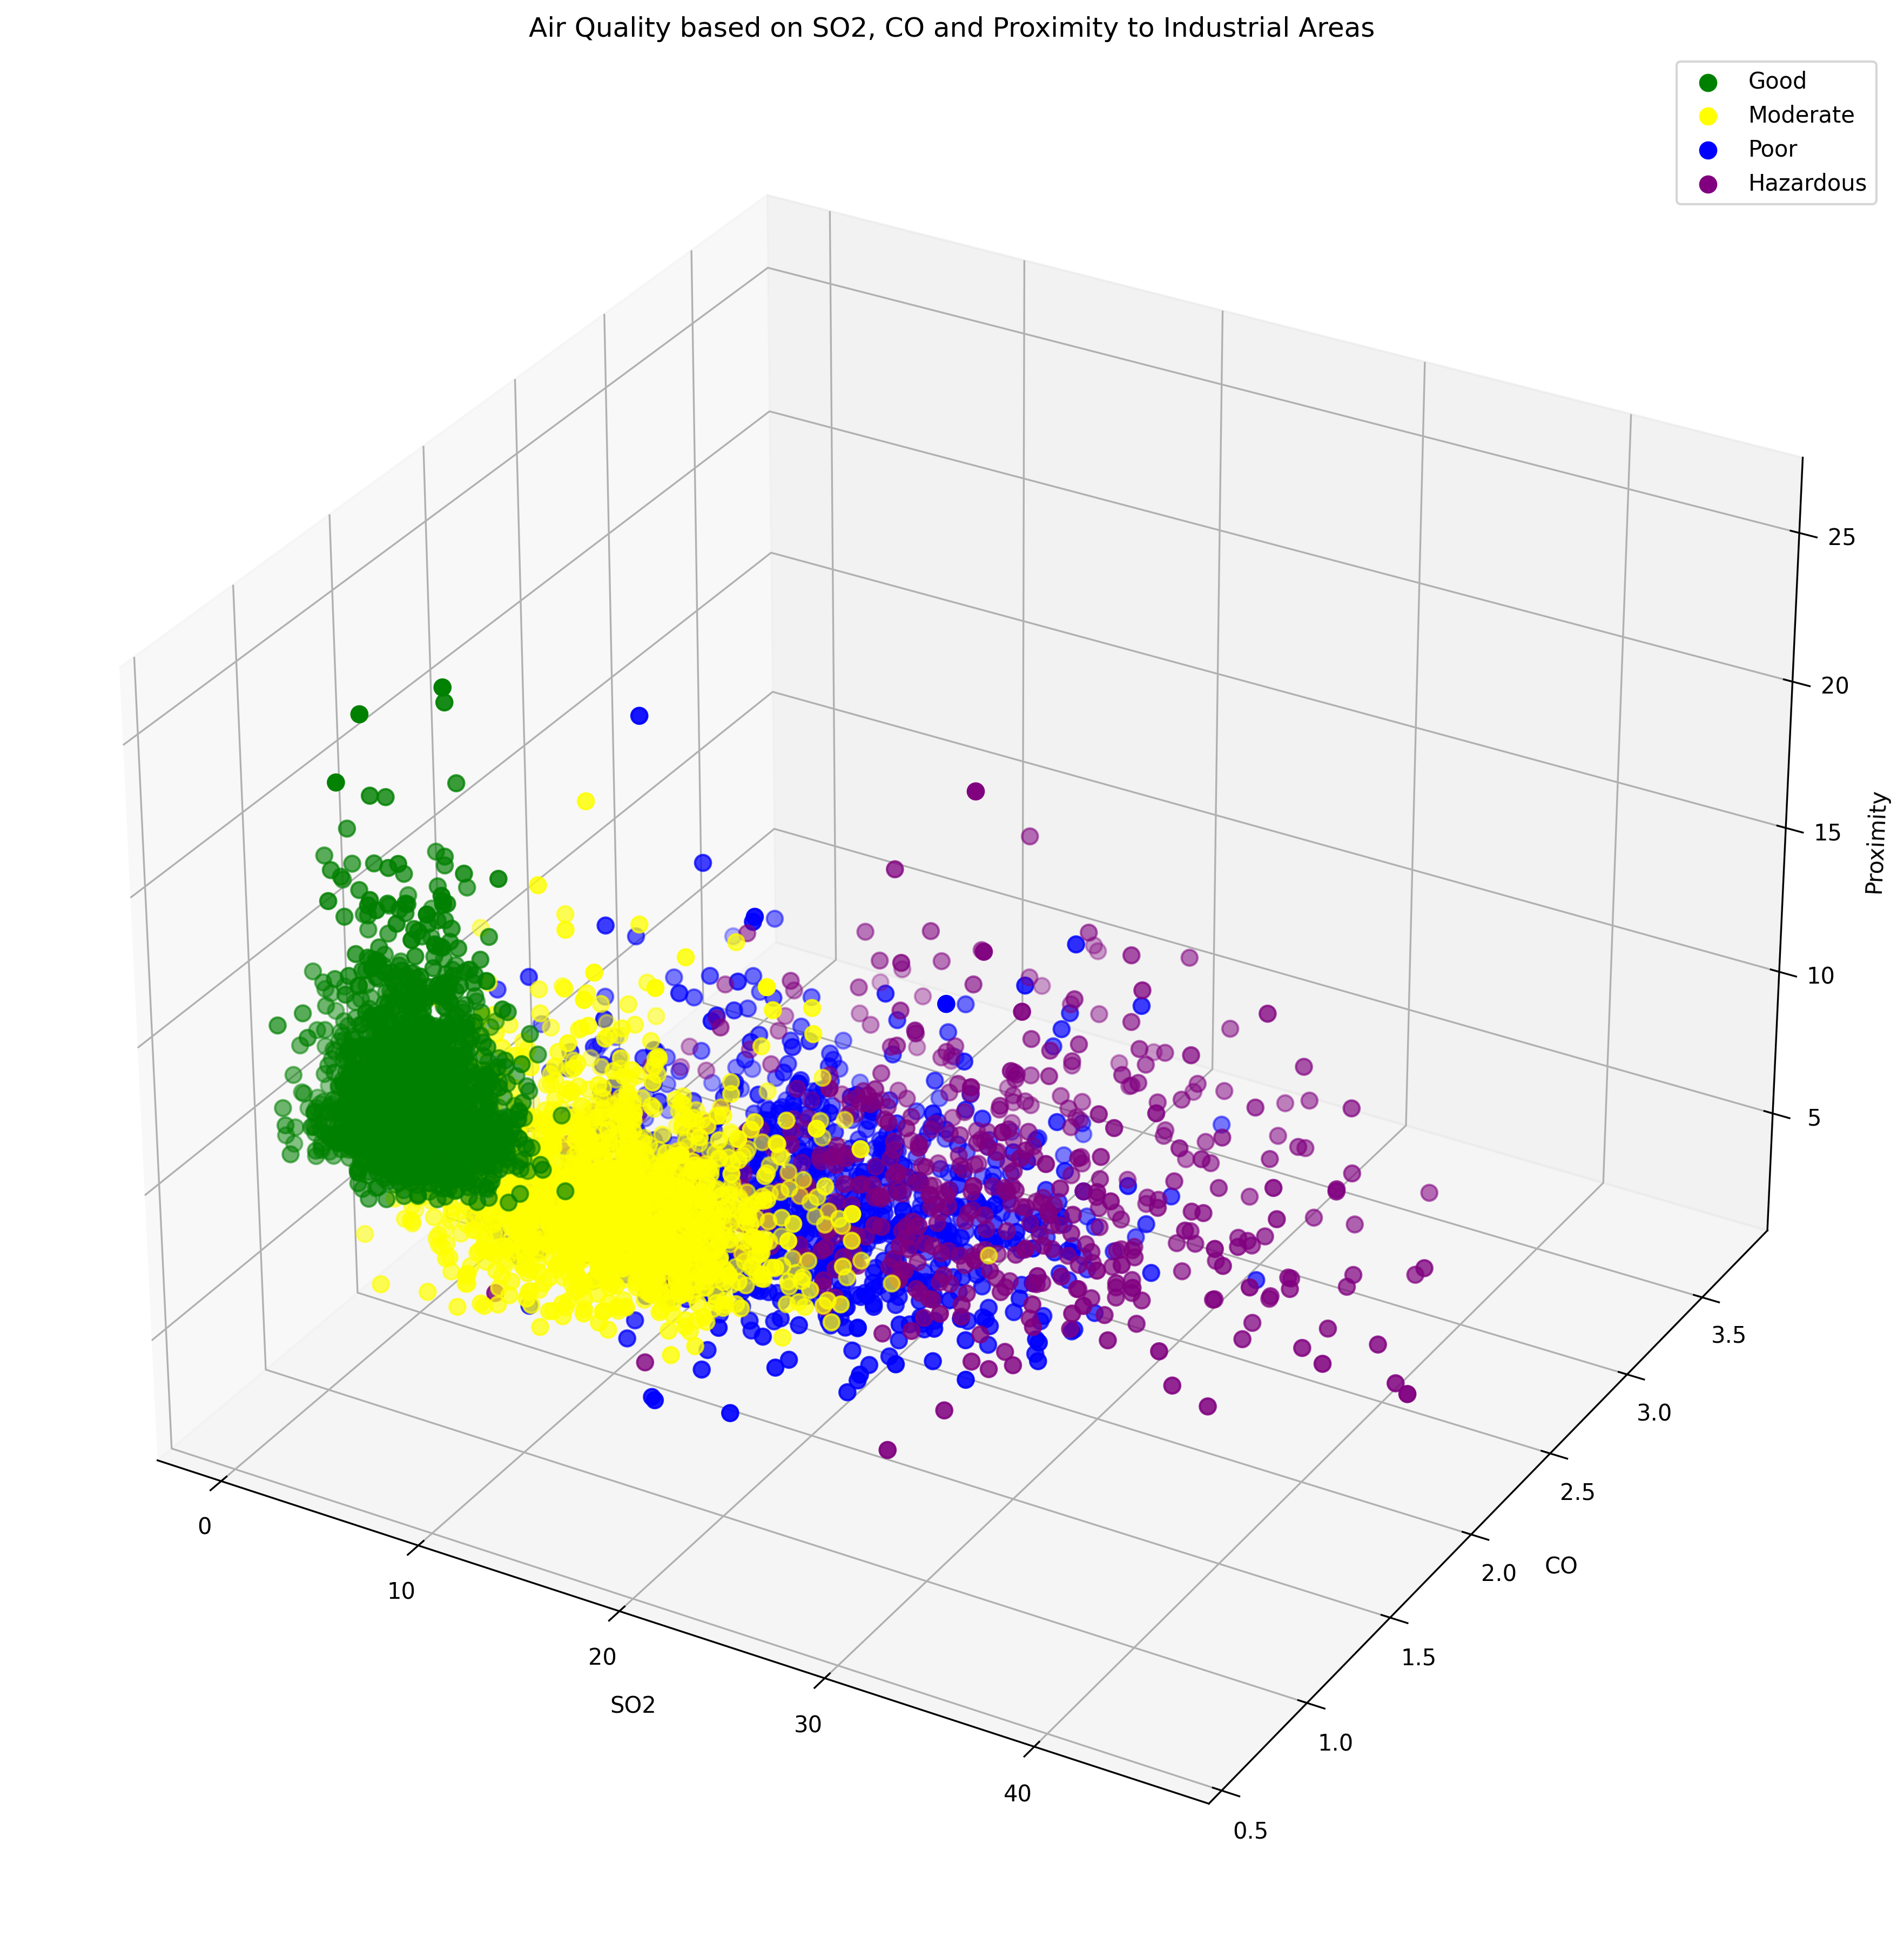
\includegraphics[width=\linewidth]{plot.png}
    \caption{{Air Quality and Pollution Assessment.}}
    \label{fig:airqual}
\end{figure}

\begin{figure}[h!]
    \centering
    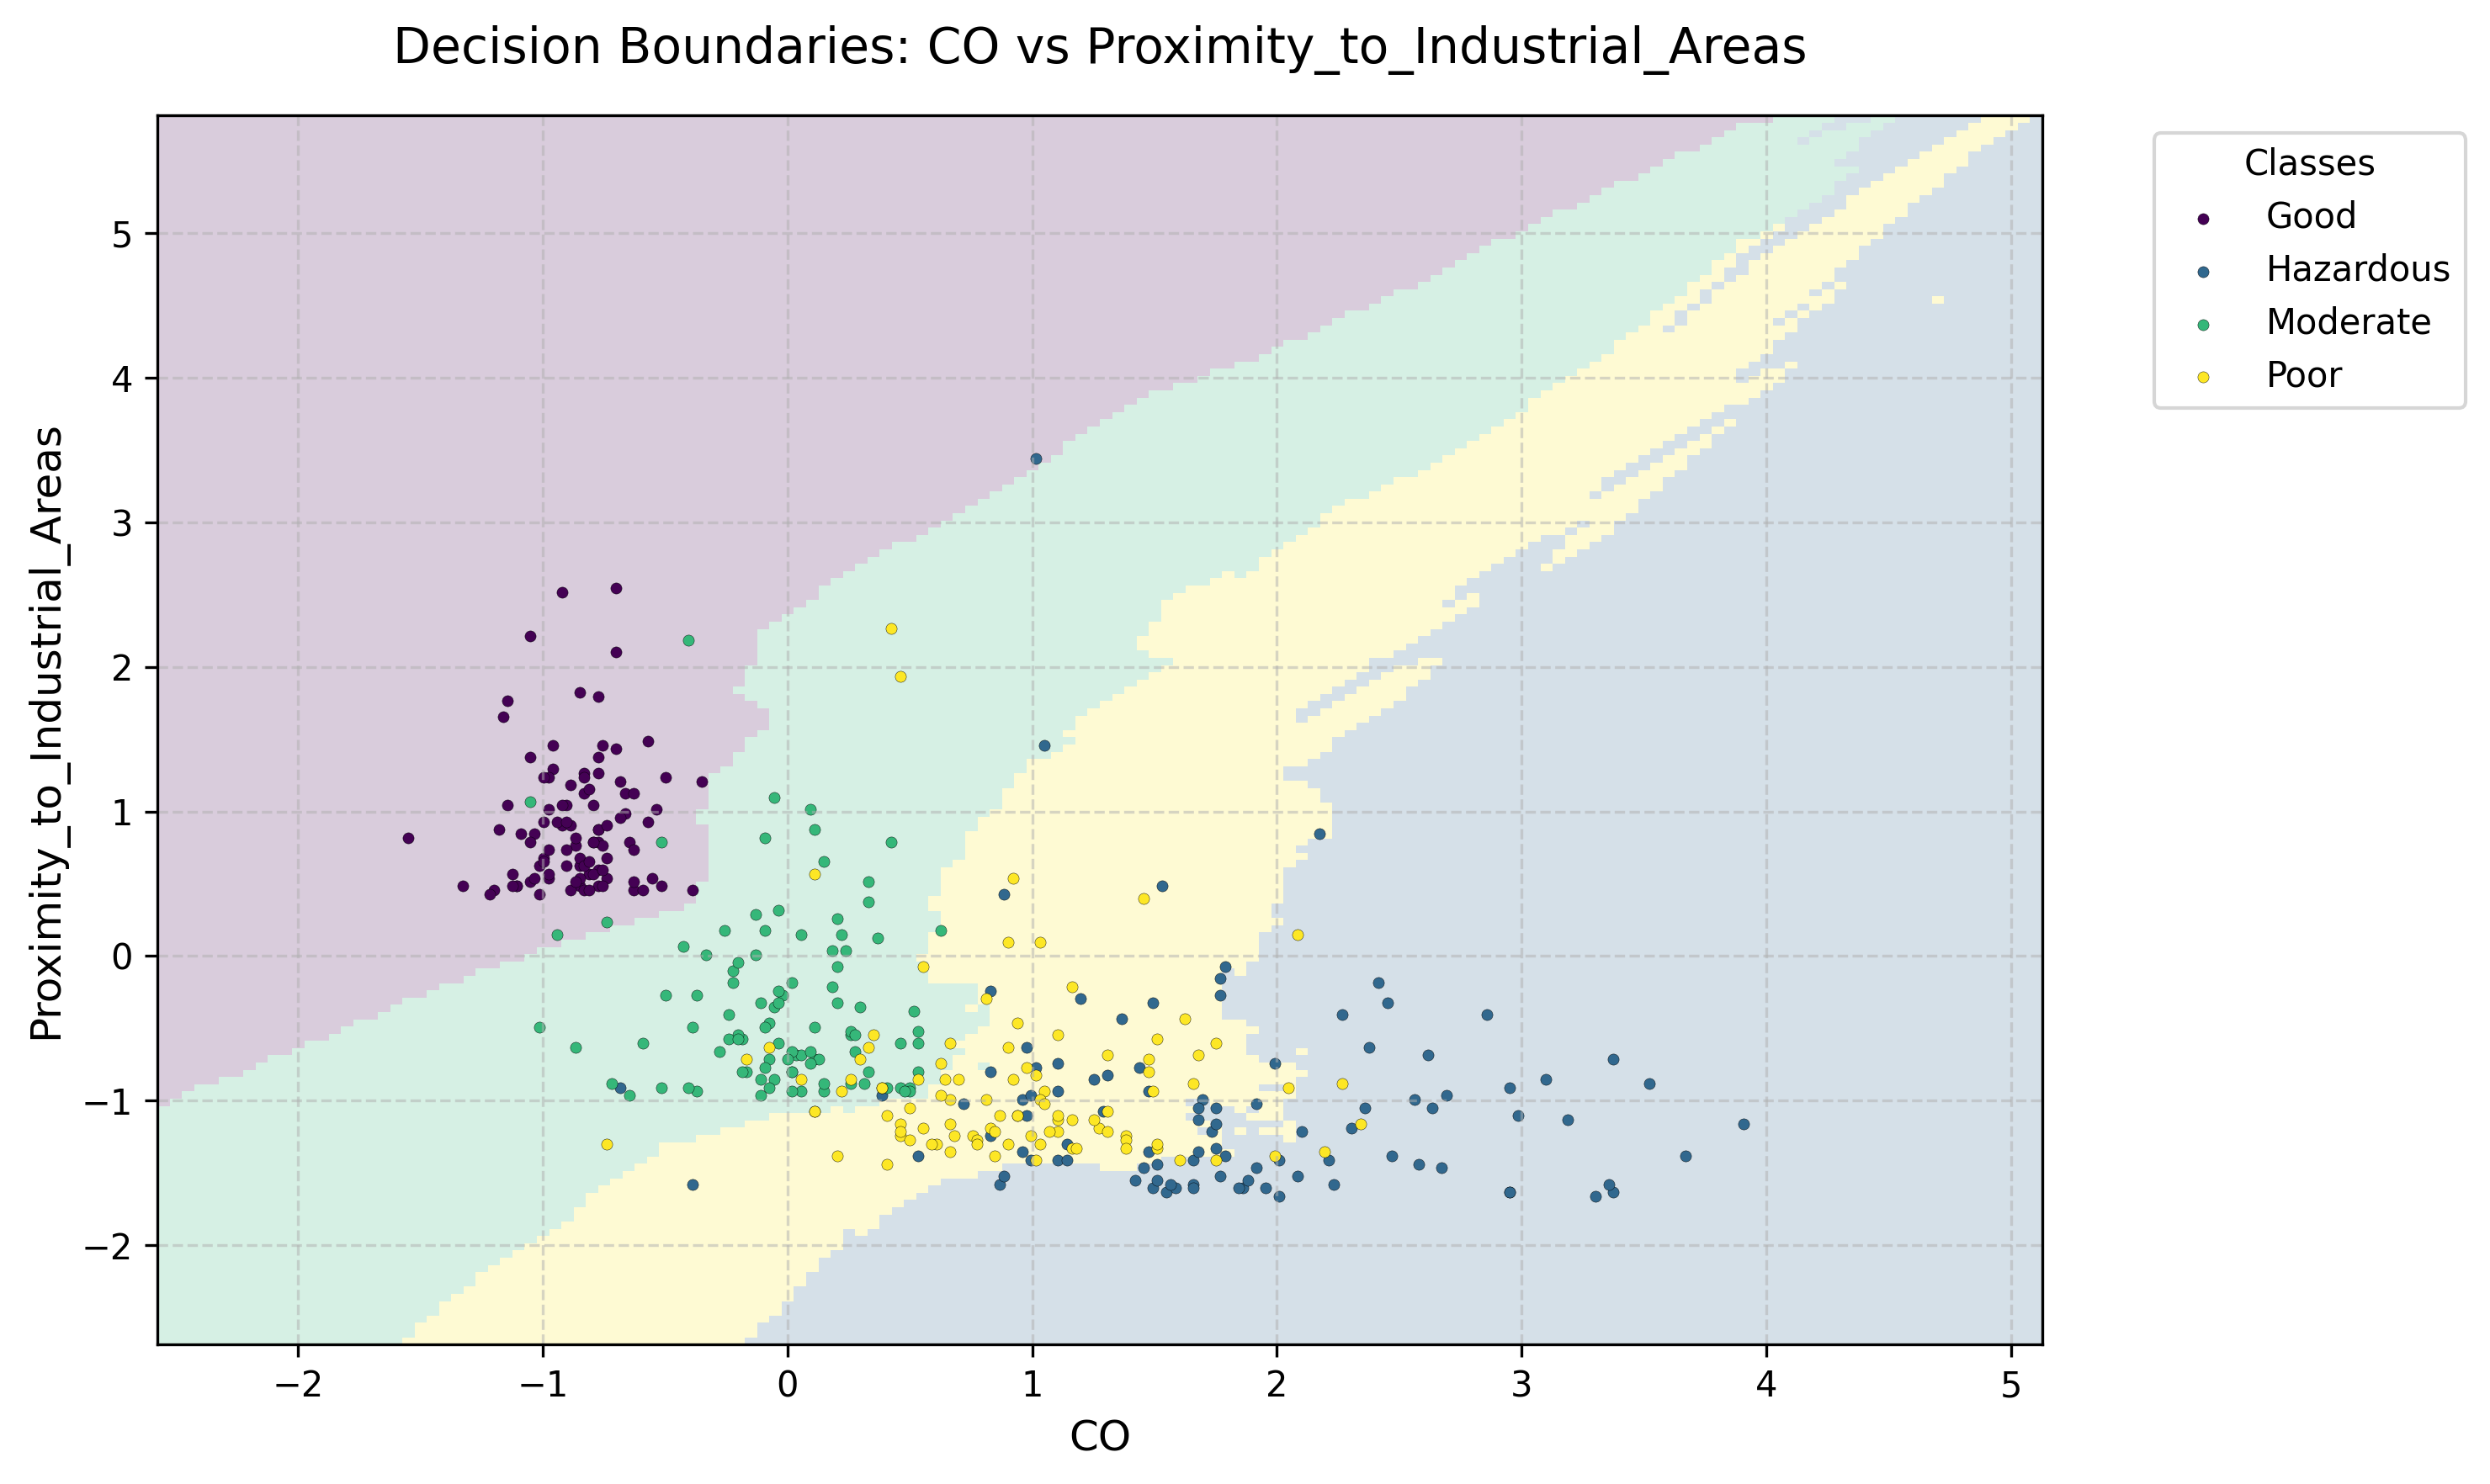
\includegraphics[width=\linewidth]{CO_Proximity_to_Industrial_Areas.png}
    \caption{\textit{Decision Boundary for CO and Proximity to Industrial Area.}}
    \label{fig:CO_Proximity}
\end{figure}

\begin{figure}[h!]
    \centering
    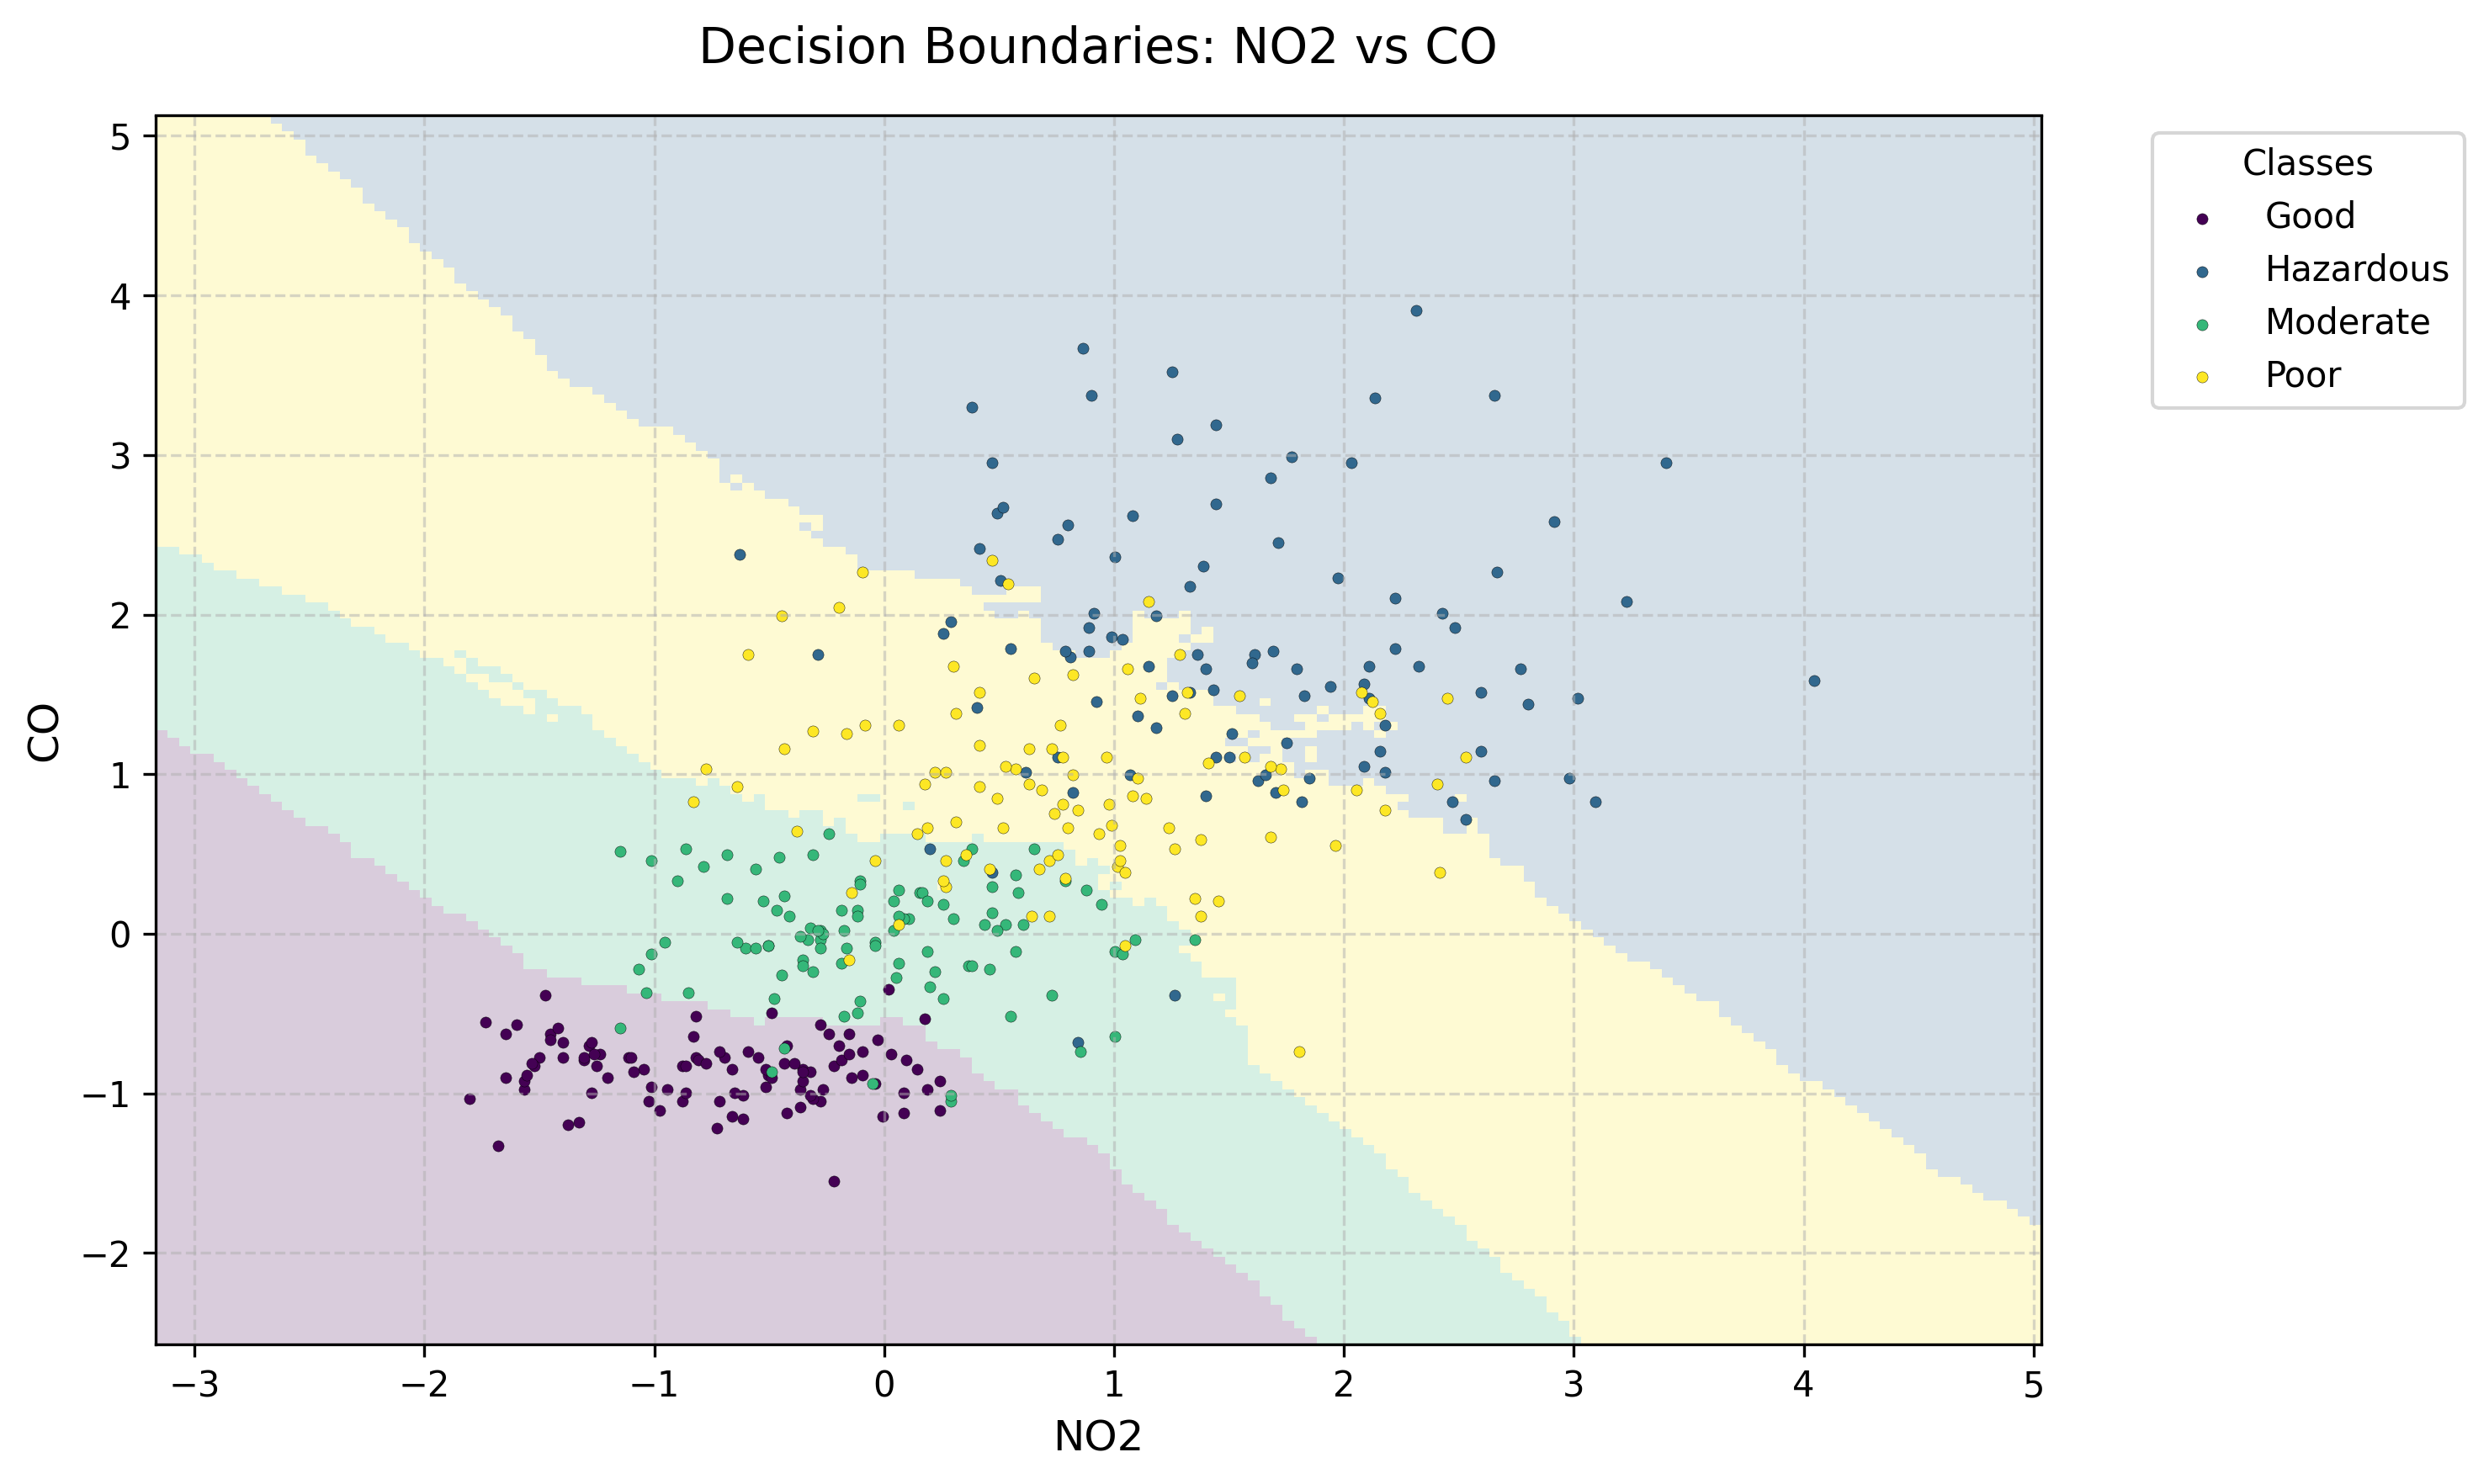
\includegraphics[width=\linewidth]{NO2_CO.png}
    \caption{\textit{Decision Boundary for NO2 and CO.}}
    \label{fig:NO2_CO}
\end{figure}

\begin{figure}[h!]
    \centering
    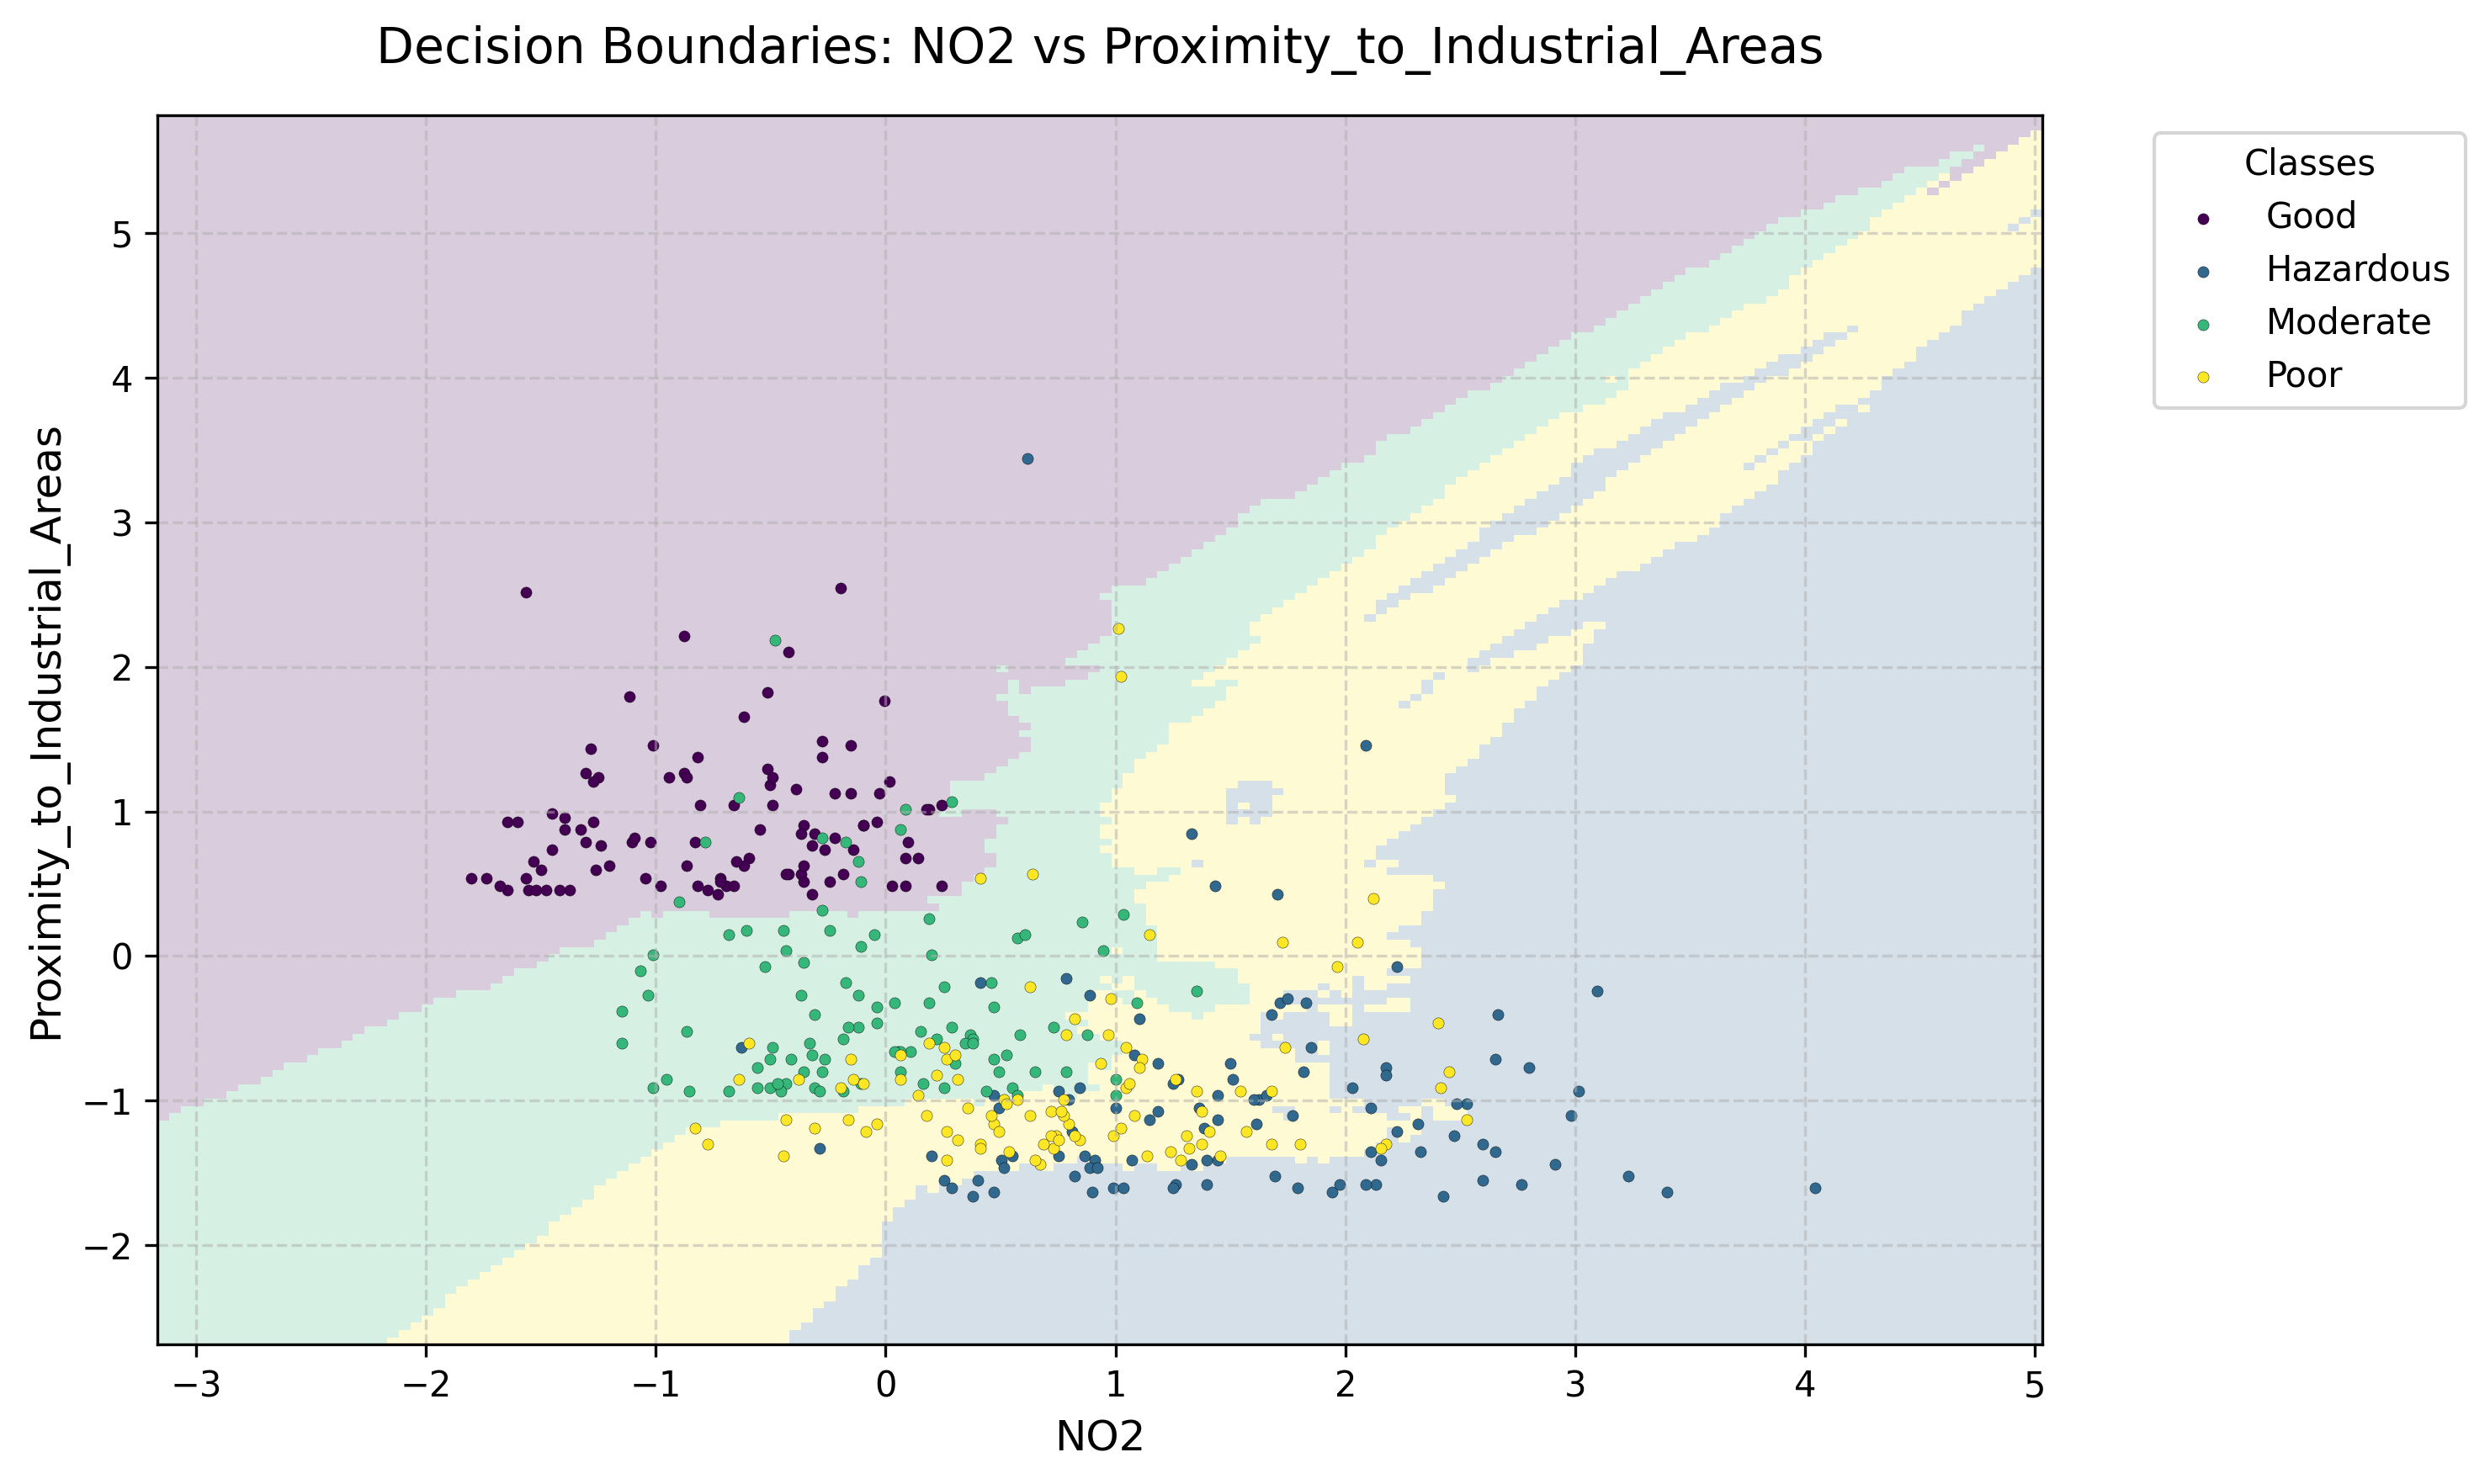
\includegraphics[width=\linewidth]{NO2_Proximity_to_Industrial_Areas.png}
    \caption{{Decision Boundary for NO2 and Proximity to Industrial Area.}}
    \label{fig:NO2_Proximity}
\end{figure}



\end{document}
